\chapter{Complex event processing}
\label{chap:cep}
%\usepackage{ amssymb }??
Chapter
\section{Formal Intro of the Event Automata}
	In our hierarchical runtime verification project, the top level of modelling is done in an event pattern language.
	This pattern language will be compiled to Calendar Event Automata.
	\subsection{Current Formalisms}
		% valami bevezeto a dologhoz?
		The two formalism we checked were the Quantified Event Automaton, and the Calendar Automaton
		\subsubsection{Event Automaton}
			% informal definition
			An Event Automaton is a non-deterministic finite-state automaton whose alphabet consists
			of parametric events and whose transitions may be labelled with guards and assignments
			
			% formal definition
			\begin{dfn}
			An EventAutomat 
			$\langle Q,A,\delta, q_0, F \rangle$ is a tuple where Q is a finite set of states, 
			$\mathcal{A} \subseteq Event$ is a finite alphabet,  %% ide nem ilyen A betut akarok!!!!
			$\delta \in (Q \times A \times Guard \times Assign \times Q)$ is a finite set of transitions, 
			$q_0 \in Q$ is an initial state, and 
			$F \subseteq Q$ is a set of final states.
			\end{dfn}
			
		\subsubsection{Calendar Event Automaton}
			% stuff about the calendar
			%informal definition of the calendar?
			In discrete event simulation, a calendar (also called event list) is a data structure that
			stores future events and the times at which these events are scheduled to occur
			
			%Formal definition of the calendar
			\begin{dfn}
			$A calendar is a finite set (or multiset) of the form C = \{ \langle e_1, t_1\rangle \, \dots ,\langle e_2, t_2\rangle \}
			where each e_i is an event and t_i is the time when event e_i is scheduled to occur. All t_is are real numbers.
			We denote by min(C) the smallest number among \{t_1,\dots ,t_n \} (with min (C) = +\infty if C is empty)
			Given a real u, we denote by Ev_u(C) the subset of C that contains all events scheduled at time u:
			
			Ev_u(C) = \{ \langle e_i, t_i \rangle  | t_i = u \wedge \langle e_i, t_i \rangle \in C \} $
			\end{dfn}
			% stuff about the calender automaton
			
	\subsection{Our Formalism}
		Akkor most tulajdonkeppen mi calendar event automatat implementaltunk :) 
\section{Examples of Event Processing}

	\subsection{File System}
	
	\begin{figure}[h]
	\centering
	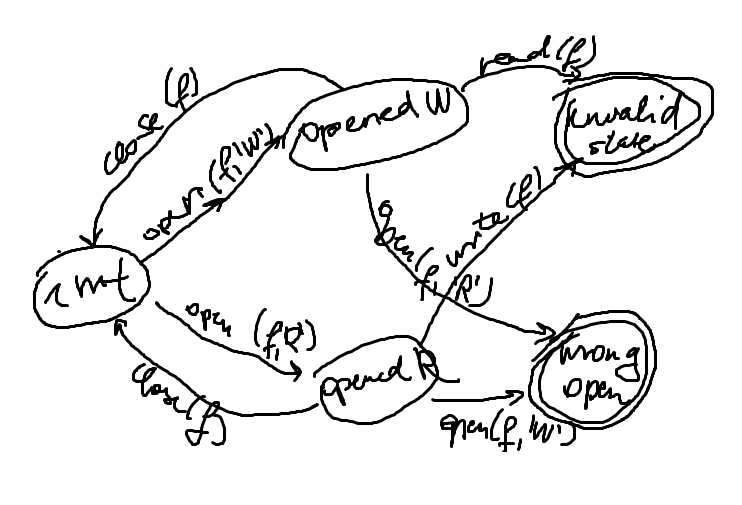
\includegraphics[width=0.5\linewidth]{include/figures/chapter_5/fileautomaton}
	\caption{Automaton of the file example}
	\label{fig:cep:fileautomaton}
	\end{figure}

	File system - A file shouldn't be read when it has been opened for Writing, and shouldn't be written, when opened for Reading. 
	A file shouldn't be opened for writing and reading without a close event between the two different opens.
	
	
	\subsection{Mars Rover Tasking - Two phase locking}

\section{Implementation}
	\subsection{Metamodel}
	%image
	\subsection{Executor}
